\def\year{2020}\relax
%File: formatting-instruction.tex
\documentclass[letterpaper]{article} % DO NOT CHANGE THIS
\usepackage{aaai20}  % DO NOT CHANGE THIS
\usepackage{times}  % DO NOT CHANGE THIS
\usepackage{helvet} % DO NOT CHANGE THIS
\usepackage{courier}  % DO NOT CHANGE THIS
\usepackage[hyphens]{url}  % DO NOT CHANGE THIS
\usepackage{graphicx} % DO NOT CHANGE THIS
\urlstyle{rm} % DO NOT CHANGE THIS
\def\UrlFont{\rm}  % DO NOT CHANGE THIS
\usepackage{graphicx}  % DO NOT CHANGE THIS
\frenchspacing  % DO NOT CHANGE THIS
\setlength{\pdfpagewidth}{8.5in}  % DO NOT CHANGE THIS
\setlength{\pdfpageheight}{11in}  % DO NOT CHANGE THIS


\def\tightlist{}

% 
% 
\usepackage{url}            % simple URL typesetting
\usepackage{booktabs}       % professional-quality tables
\usepackage{amsfonts}       % blackboard math symbols
\usepackage{nicefrac}       % compact symbols for 1/2, etc.
\usepackage{microtype}      % microtypography
% 
% 
% 
\usepackage{amsmath}
\usepackage{amsthm}
\usepackage{latexsym}
\usepackage{amssymb}
\usepackage{amsbsy}
\usepackage{graphics}
\usepackage{epsfig}


%\nocopyright
%PDF Info Is REQUIRED.
% For /Author, add all authors within the parentheses, separated by commas. No accents or commands.
% For /Title, add Title in Mixed Case. No accents or commands. Retain the parentheses.
 \pdfinfo{
/Title (The hidden manifold distance for functional data)
/Author (Susan Wei and Marie-H\'el\`{e}ne Descary)
} %Leave this	
% /Title ()
% Put your actual complete title (no codes, scripts, shortcuts, or LaTeX commands) within the parentheses in mixed case
% Leave the space between \Title and the beginning parenthesis alone
% /Author ()
% Put your actual complete list of authors (no codes, scripts, shortcuts, or LaTeX commands) within the parentheses in mixed case. 
% Each author should be only by a comma. If the name contains accents, remove them. If there are any LaTeX commands, 
% remove them. 

% DISALLOWED PACKAGES
% \usepackage{authblk} -- This package is specifically forbidden
% \usepackage{balance} -- This package is specifically forbidden
% \usepackage{caption} -- This package is specifically forbidden
% \usepackage{color (if used in text)
% \usepackage{CJK} -- This package is specifically forbidden
% \usepackage{float} -- This package is specifically forbidden
% \usepackage{flushend} -- This package is specifically forbidden
% \usepackage{fontenc} -- This package is specifically forbidden
% \usepackage{fullpage} -- This package is specifically forbidden
% \usepackage{geometry} -- This package is specifically forbidden
% \usepackage{grffile} -- This package is specifically forbidden
% \usepackage{hyperref} -- This package is specifically forbidden
% \usepackage{navigator} -- This package is specifically forbidden
% (or any other package that embeds links such as navigator or hyperref)
% \indentfirst} -- This package is specifically forbidden
% \layout} -- This package is specifically forbidden
% \multicol} -- This package is specifically forbidden
% \nameref} -- This package is specifically forbidden
% \natbib} -- This package is specifically forbidden -- use the following workaround:
%\newcommand{\citet}[1]{\citeauthor{#1} \shortcite{#1}} 
%\newcommand{\citep}{\cite} 
%\newcommand{\citealp}[1]{\citeauthor{#1} \citeyear{#1}}
% \usepackage{savetrees} -- This package is specifically forbidden
% \usepackage{setspace} -- This package is specifically forbidden
% \usepackage{stfloats} -- This package is specifically forbidden
% \usepackage{tabu} -- This package is specifically forbidden
% \usepackage{titlesec} -- This package is specifically forbidden
% \usepackage{tocbibind} -- This package is specifically forbidden
% \usepackage{ulem} -- This package is specifically forbidden
% \usepackage{wrapfig} -- This package is specifically forbidden
% DISALLOWED COMMANDS
% \nocopyright -- Your paper will not be published if you use this command
% \addtolength -- This command may not be used
% \balance -- This command may not be used
% \baselinestretch -- Your paper will not be published if you use this command
% \clearpage -- No page breaks of any kind may be used for the final version of your paper
% \columnsep -- This command may not be used
% \newpage -- No page breaks of any kind may be used for the final version of your paper
% \pagebreak -- No page breaks of any kind may be used for the final version of your paperr
% \pagestyle -- This command may not be used
% \tiny -- This is not an acceptable font size.
% \vspace{- -- No negative value may be used in proximity of a caption, figure, table, section, subsection, subsubsection, or reference
% \vskip{- -- No negative value may be used to alter spacing above or below a caption, figure, table, section, subsection, subsubsection, or reference

\setcounter{secnumdepth}{0} %May be changed to 1 or 2 if section numbers are desired.

% The file aaai20.sty is the style file for AAAI Press 
% proceedings, working notes, and technical reports.
%
\setlength\titlebox{2.5in} % If your paper contains an overfull \vbox too high warning at the beginning of the document, use this
% command to correct it. You may not alter the value below 2.5 in
\title{The Hidden Manifold Distance for Functional Data}
%Your title must be in mixed case, not sentence case. 
% That means all verbs (including short verbs like be, is, using,and go), 
% nouns, adverbs, adjectives should be capitalized, including both words in hyphenated terms, while
% articles, conjunctions, and prepositions are lower case unless they
% directly follow a colon or long dash



% \author{Susan Wei\textsuperscript{\rm 1} and Marie-H\'el\`{e}ne Descary\textsuperscript{\rm 2}\\ % All authors must be
% \textsuperscript{\rm 1} The University of Melbourne, \textsuperscript{\rm 2}Universit\'e du Qu\'ebec \`{a} Montr\'eal\\ }

%in the same font size and format. Use \Large and \textbf to achieve this result when breaking a line

%If you have multiple authors and multiple affiliations
% use superscripts in text and roman font to identify them. For example, Sunil Issar,\textsuperscript{\rm 2} J. Scott Penberthy\textsuperscript{\rm 3} George Ferguson,\textsuperscript{\rm 4} Hans Guesgen\textsuperscript{\rm 5}. Note that the comma should be placed BEFORE the superscript for optimum readability
 % email address must be in roman text type, not monospace or sans serif

\begin{document}

\maketitle

\begin{abstract}
In many machine learning applications, the observed data is a
discretely-sampled realisation of a continuous process. While one can
naively treat such data as vectors in Euclidean space, one may do better
to regard them as functional data.  
When the underlying curves of interest lie on a manifold, e.g.~probability density
functions or warped curves of a common template function, there is further structure to exploit. 
This work addresses the estimation of pairwise geodesic
distances between functional manifold data that are observed with noise,
causing them to lie off the manifold. This setting falls outside of
classic manifold learning techniques which require data to live exactly
on or very near a manifold. The proposed methodology first sends the
observed functional data to the hidden manifold, estimated using
subspace-constrained mean-shift. Geodesic distances are subsequently
calculated by employing shortest-path algorithms on this estimated
manifold. Improved estimation of the pairwise geodesic distance has
potential benefits for downstream tasks such as distance-based functional classification.
\end{abstract}

\documentclass[]{article}
\usepackage{lmodern}
\usepackage{amssymb,amsmath}
\usepackage{ifxetex,ifluatex}
\usepackage{fixltx2e} % provides \textsubscript
\ifnum 0\ifxetex 1\fi\ifluatex 1\fi=0 % if pdftex
  \usepackage[T1]{fontenc}
  \usepackage[utf8]{inputenc}
\else % if luatex or xelatex
  \ifxetex
    \usepackage{mathspec}
  \else
    \usepackage{fontspec}
  \fi
  \defaultfontfeatures{Ligatures=TeX,Scale=MatchLowercase}
\fi
% use upquote if available, for straight quotes in verbatim environments
\IfFileExists{upquote.sty}{\usepackage{upquote}}{}
% use microtype if available
\IfFileExists{microtype.sty}{%
\usepackage{microtype}
\UseMicrotypeSet[protrusion]{basicmath} % disable protrusion for tt fonts
}{}
\usepackage[margin=1in]{geometry}
\usepackage{hyperref}
\hypersetup{unicode=true,
            pdftitle={The hidden manifold distance for functional data},
            pdfborder={0 0 0},
            breaklinks=true}
\urlstyle{same}  % don't use monospace font for urls
\usepackage{color}
\usepackage{fancyvrb}
\newcommand{\VerbBar}{|}
\newcommand{\VERB}{\Verb[commandchars=\\\{\}]}
\DefineVerbatimEnvironment{Highlighting}{Verbatim}{commandchars=\\\{\}}
% Add ',fontsize=\small' for more characters per line
\usepackage{framed}
\definecolor{shadecolor}{RGB}{248,248,248}
\newenvironment{Shaded}{\begin{snugshade}}{\end{snugshade}}
\newcommand{\AlertTok}[1]{\textcolor[rgb]{0.94,0.16,0.16}{#1}}
\newcommand{\AnnotationTok}[1]{\textcolor[rgb]{0.56,0.35,0.01}{\textbf{\textit{#1}}}}
\newcommand{\AttributeTok}[1]{\textcolor[rgb]{0.77,0.63,0.00}{#1}}
\newcommand{\BaseNTok}[1]{\textcolor[rgb]{0.00,0.00,0.81}{#1}}
\newcommand{\BuiltInTok}[1]{#1}
\newcommand{\CharTok}[1]{\textcolor[rgb]{0.31,0.60,0.02}{#1}}
\newcommand{\CommentTok}[1]{\textcolor[rgb]{0.56,0.35,0.01}{\textit{#1}}}
\newcommand{\CommentVarTok}[1]{\textcolor[rgb]{0.56,0.35,0.01}{\textbf{\textit{#1}}}}
\newcommand{\ConstantTok}[1]{\textcolor[rgb]{0.00,0.00,0.00}{#1}}
\newcommand{\ControlFlowTok}[1]{\textcolor[rgb]{0.13,0.29,0.53}{\textbf{#1}}}
\newcommand{\DataTypeTok}[1]{\textcolor[rgb]{0.13,0.29,0.53}{#1}}
\newcommand{\DecValTok}[1]{\textcolor[rgb]{0.00,0.00,0.81}{#1}}
\newcommand{\DocumentationTok}[1]{\textcolor[rgb]{0.56,0.35,0.01}{\textbf{\textit{#1}}}}
\newcommand{\ErrorTok}[1]{\textcolor[rgb]{0.64,0.00,0.00}{\textbf{#1}}}
\newcommand{\ExtensionTok}[1]{#1}
\newcommand{\FloatTok}[1]{\textcolor[rgb]{0.00,0.00,0.81}{#1}}
\newcommand{\FunctionTok}[1]{\textcolor[rgb]{0.00,0.00,0.00}{#1}}
\newcommand{\ImportTok}[1]{#1}
\newcommand{\InformationTok}[1]{\textcolor[rgb]{0.56,0.35,0.01}{\textbf{\textit{#1}}}}
\newcommand{\KeywordTok}[1]{\textcolor[rgb]{0.13,0.29,0.53}{\textbf{#1}}}
\newcommand{\NormalTok}[1]{#1}
\newcommand{\OperatorTok}[1]{\textcolor[rgb]{0.81,0.36,0.00}{\textbf{#1}}}
\newcommand{\OtherTok}[1]{\textcolor[rgb]{0.56,0.35,0.01}{#1}}
\newcommand{\PreprocessorTok}[1]{\textcolor[rgb]{0.56,0.35,0.01}{\textit{#1}}}
\newcommand{\RegionMarkerTok}[1]{#1}
\newcommand{\SpecialCharTok}[1]{\textcolor[rgb]{0.00,0.00,0.00}{#1}}
\newcommand{\SpecialStringTok}[1]{\textcolor[rgb]{0.31,0.60,0.02}{#1}}
\newcommand{\StringTok}[1]{\textcolor[rgb]{0.31,0.60,0.02}{#1}}
\newcommand{\VariableTok}[1]{\textcolor[rgb]{0.00,0.00,0.00}{#1}}
\newcommand{\VerbatimStringTok}[1]{\textcolor[rgb]{0.31,0.60,0.02}{#1}}
\newcommand{\WarningTok}[1]{\textcolor[rgb]{0.56,0.35,0.01}{\textbf{\textit{#1}}}}
\usepackage{graphicx,grffile}
\makeatletter
\def\maxwidth{\ifdim\Gin@nat@width>\linewidth\linewidth\else\Gin@nat@width\fi}
\def\maxheight{\ifdim\Gin@nat@height>\textheight\textheight\else\Gin@nat@height\fi}
\makeatother
% Scale images if necessary, so that they will not overflow the page
% margins by default, and it is still possible to overwrite the defaults
% using explicit options in \includegraphics[width, height, ...]{}
\setkeys{Gin}{width=\maxwidth,height=\maxheight,keepaspectratio}
\IfFileExists{parskip.sty}{%
\usepackage{parskip}
}{% else
\setlength{\parindent}{0pt}
\setlength{\parskip}{6pt plus 2pt minus 1pt}
}
\setlength{\emergencystretch}{3em}  % prevent overfull lines
\providecommand{\tightlist}{%
  \setlength{\itemsep}{0pt}\setlength{\parskip}{0pt}}
\setcounter{secnumdepth}{5}
% Redefines (sub)paragraphs to behave more like sections
\ifx\paragraph\undefined\else
\let\oldparagraph\paragraph
\renewcommand{\paragraph}[1]{\oldparagraph{#1}\mbox{}}
\fi
\ifx\subparagraph\undefined\else
\let\oldsubparagraph\subparagraph
\renewcommand{\subparagraph}[1]{\oldsubparagraph{#1}\mbox{}}
\fi

%%% Use protect on footnotes to avoid problems with footnotes in titles
\let\rmarkdownfootnote\footnote%
\def\footnote{\protect\rmarkdownfootnote}

%%% Change title format to be more compact
\usepackage{titling}

% Create subtitle command for use in maketitle
\providecommand{\subtitle}[1]{
  \posttitle{
    \begin{center}\large#1\end{center}
    }
}

\setlength{\droptitle}{-2em}

  \title{The hidden manifold distance for functional data}
    \pretitle{\vspace{\droptitle}\centering\huge}
  \posttitle{\par}
    \author{}
    \preauthor{}\postauthor{}
    \date{}
    \predate{}\postdate{}
  

\begin{document}
\maketitle

\newcommand {\To}{\rightarrow}
\newcommand {\TO}{\Rightarrow}
\newcommand {\R}{\mathbb{R}}
\newcommand {\Prob}{\mathbb{P}}
\newcommand{\E}{\mathbb{E}}
\newcommand {\cov}{\textrm{Cov}}
\newcommand {\var}{\textrm{Var}}
\newcommand {\1}{\textrm{\textbf{1}}}
\newcommand{\M}{\mathcal{M}}

\hypertarget{abstract}{%
\section{Abstract}\label{abstract}}

Functional data analysis is the statistical analysis of smooth
infinite-dimensional curves. The challenge of analyzing
infinite-dimensional objects is ameliorated by the fact that, since
observations are smooth over their domain, the dimensionality of the
curves is only artifically high. Less studied in functional data
analysis is the idea that the curves may actually live in a submanifold
with low intrinsic dimension. Interesting classes of functional manifold
data include the class of probability density functions and the class of
warped curves of a common template function. Since these spaces are not
vector spaces, even basic operations such as addition and subtraction
require special consideration. In this work we set ourselves the task of
calculating the pairwise geodesic distance between functional
observations that, due to noise, live near a non-linear manifold rather
than exactly on the manifold. We will show that good estimation of the
geodesic distance cannot be accomplished by naive methods such as
smoothing followed by a shortest-path algorithm. Instead, we propose a
dedicated technique for pairwise geodesic distance estimation by first
projecting the functional data to the underlying hidden manifold and
then perofrming operations on this hidden manifold. We conclude the work
by showing the implications for many downstream tasks in functional data
analysis, in particular distanced-based functional classification.

\hypertarget{introduction-susan}{%
\section{Introduction {[}Susan{]}}\label{introduction-susan}}

Let \(X_1,\ldots,X_n\) be a sample of \(n\) independant realizations of
a random variable \(X\) that takes value in the Hilbert space
\(L^2([a,b],\mathbb{R})\). We additionally assume that the function
\(X\) belongs to a low-dimensional nonlinear manifold
\(\mathcal{M}\subset L^2([a,b],\mathbb{R})\), in which case a geodesic
distance taking into account the intrinsic structure of \(\mathcal{M}\)
rather than the \(L^2\) distance should be used as a measure of distance
between two functions in \(\mathcal{M}\). As many statistical methods
depend on some measure of distance, downstream benefits of using the
geodesic distance can be expected.

???insert example that shows pairwise geodesic distances give visually
more interesting results than pairwise \(L_2\) distance.???

Given perfect functional observations, i.e.~with no measurement error
and on a very dense domain grid, the estimation of the geodesic distance
can be accomplished straightforwardly using algorithms such as Floyd's.
However, functional data are observed with noise in such a way that the
observed functional data no longer live on a manifold. Though powerful
techniques exist for smoothing discretely observed noisy functional
data, the smoothing is designed for the \(L_2\) recovery of the original
curve, not to ensure the recovered functional versions of the data lie
on or close to the functional manifold \(\mathcal{M}\).

With this challenge in mind, we put forth a technique for the specific
task of estimating pairwise geodesic distances
\(\{ d_\mathcal{M}(X_i,X_j\}_{i>j}\), to be defined when we have access
only to discretely-observed noisy functional observations that possibly
live off the true manifold. Briefly outline the methodology: MDS plus
density ridge are used in a cool way to estimate (consistently?, let's
hope..) pairwise geodesic distances.

\hypertarget{related-work-susan}{%
\subsection{Related Work {[}Susan{]}}\label{related-work-susan}}

(Chen and Muller 2012)

(Lin and Yao 2017)

(Dimeglio et al. 2014)

\hypertarget{setting-susan}{%
\subsection{Setting {[}Susan{]}}\label{setting-susan}}

Let \(X_1,\ldots,X_n\) be independent realizations of a random function
\(X\in\mathcal{M}\subset L^2([a,b],\mathbb{R})\), where \(\mathcal{M}\)
is an unknown manifold. Suppose that each curve \(X_i\) is observed with
measurements errors on a grid \(T_i=(t_{i1},\ldots,t_{iK})\), i.e.~we
observe a sample of \(K\)-dimensional vectors \(Y_1,\ldots,Y_n\) with
\(Y_{ij} = X_i(t_{ij}) + \epsilon_{ij}\), where the random variables
\(\epsilon_{ij}\) are of mean zero and uncorrelated with each other. We
assume that the grids \(T_1,\ldots,T_n\) are dense.

Let \(\tilde X_1,\ldots,\tilde X_n\) denote the functional versions of
the raw data by some smoothing method. Our proposed methodology is
unspecific to the smoothing method employed. For simplicity however,
let's say we employ spline smoothing to recover the functional versions
of the raw data, i.e.\\
\[ \tilde X_i = \arg\min_{f\in C^2[0,1]}\left\{\sum_{j=1}^{K}\left(f(t_{ij})-Y_{ij}\right)^2+\lambda \|\partial^2_tf\|^2_{L^2}\right\}\]
where \(\lambda>0\) is a tuning parameter controlling the smoothness of
\(\tilde X_i\).

\hypertarget{relevant-differential-geometry-concepts-susan}{%
\subsection{Relevant differential geometry concepts
{[}Susan{]}}\label{relevant-differential-geometry-concepts-susan}}

We first rigorously define the concepts of geodesic and geodesic
distance. Following (Lin et al. 2014), let \((\mathcal{M},g)\) be a
\(d\)-dimensional Riemannian manifold, where \(g\) is a Riemannian
metric tensor on \(\mathcal{M}\) which can be used to assign a metric on
the manifold. Specifically, for each point \(p\) on the manifold, the
Riemannian metric tensor \(g\) has an inner product \(g_p\) on the
tangent space \(T_p \mathcal{M}\). The norm of a tangent vector
\(v \in T_p \mathcal{M}\) is defined as \[||v|| = \sqrt{g_p(v,v)}.\] If
\(\gamma: [a,b] \subset \mathbb{R}\to \mathcal{M}\) is a smooth curve,
its length is then defined as
\[ l(\gamma) := \int_a^b || \frac{\,d\gamma}{\,d t}(t) || \,dt .\] The
geodesic distance between two points \(p,q\) on the manifold
\(\mathcal{M}\), based on this metric tensor \(g\), is defined as
\[ d_g(p,q):=\inf \{l(\gamma): \gamma:[a,b] \to \mathcal{M}\text{ piecewise smooth}, \gamma(a) = p, \gamma(b) = q]  \}.\]

\hypertarget{proposed-method-for-estimating-geodesic-distances-marie}{%
\section{Proposed method for estimating geodesic distances
{[}Marie{]}}\label{proposed-method-for-estimating-geodesic-distances-marie}}

We first describe an important helper algorithm which we call IsoGeo. It
is a subroutine of the classic Isomap procedure. Isomap is a three steps
procedure that takes as input a set of points
\(x_1,\ldots,x_n\in \mathbb{R}^D\) and produces an embedding of the
input data in the space \(\mathbb{R}^d\) with \(d<D\), that preserves
pairwise geodesic distances.

\begin{enumerate}
\item The first step consists in constructing a weighted graph $G$ with nodes corresponding to the input data and for which the weight of an edge between two nodes $x_i$ and $x_j$ is equal to $||x_i-x_j ||_{\mathbb{R}^D}$. The graph $G$ is constructed such that a node is connected to a fix number $N$ of neighbors or to all nodes that are at a distance smaller than a given value $\epsilon$.
\item In the second step, the pairwise geodesic distances $d_\mathcal{M}(x_i,x_j)$
are estimated based on $G$. The geodesic distance between two nodes is simply the length of the shortest path in $G$ between these two nodes, which we calculate with the Floyd-Warshall algorithm [@Warshall1962]
<!-- or Dijkstra’s  which one do we actually use in our implementation, the FW or D? -->
\item The last step consists in using MDS on the matrix of pairwise geodesic distances obtained in the first step in order to obtain an embedding in $\mathbb{R}^d$.
\end{enumerate}

In what follows, we call IsoGeo the procedure of estimating pairwise
geodesic distances with the two first steps of Isomap. Note that Floyd
or Dijkstra are methods to find the smallest path given a weigthed graph
but they are not related to how to calculate that graph (which is the
difficult part, depend on number of neighbors, many method out there to
calculate that graph in a robust way, P-ISOMAP is one of these).

Our method is described by the following steps:

\begin{enumerate}
\def\labelenumi{\arabic{enumi}.}
\setcounter{enumi}{1}
\tightlist
\item
  Obtain a \(s\)-dimensional representation
  \(\tilde X^s_1,\ldots,\tilde X^s_n\) of the functions
  \(\tilde X_1,\ldots,\tilde X_n\) that ``preserves'' the pairwise
  \(L^2\) distances by using MDS.
\item
  Obtain
  \(\tilde X^{s,\hat \mathcal{M}}_1,\ldots,\tilde X^{s,\hat \mathcal{M}}_n\)
  a ``projection'' of \(\tilde X^s_1,\ldots,\tilde X^s_n\) onto a ridge
  \(\hat \mathcal{M}\) which is computed with the subspace constrained
  mean-shift algorithm (Ozertem and Erdogmus 2011).
\item
  Use IsoGeo to approximate the pairwise geodesic distances
  \(\{d_{\hat \mathcal{M}}(\tilde X^{s,\hat \mathcal{M}}_i,\tilde X^{s,\hat \mathcal{M}}_j)\}_{i>j}\)
  and define the \(n\) by \(n\) matrix \[
  \hat G(i,j)=\hat G(j,i) = \left\{ \begin{array}{ll}
   d_{\hat \mathcal{M}}(\tilde X^{s,\hat \mathcal{M}}_i,\tilde X^{s,\hat \mathcal{M}}_j) & \textrm{if $i\neq j$,}\\
   0 & \textrm{otherwise.}
    \end{array} \right.
  \]
\end{enumerate}

Since the ridge estimation obtained from noisy measurements of a
manifold should approximate well the manifold (Genovese et al. 2014), we
expect the points
\(\tilde X^{s,\hat \mathcal{M}}_1,\ldots,\tilde X^{s,\hat \mathcal{M}}_n\)
to lie close to the real manifold \(\mathcal{M}\) and then
\(d_{\hat \mathcal{M}}\) to be close to \(d_\mathcal{M}\). Ridge
estimation suffers from the curse of dimensionality, this is why we
first reduce the dimension of our data with MDS and then apply the
shift-mean algorithm to estimate the ridge.

\hypertarget{selection-of-tuning-parameters-marie}{%
\subsection{Selection of tuning parameters
{[}Marie{]}}\label{selection-of-tuning-parameters-marie}}

Describe heuristics. We pick the bandwidth \(h\) in the subspace
constrained mean-shift using Equation (A1) of (Chen et al. 2015).

\hypertarget{simulation-study}{%
\section{Simulation study}\label{simulation-study}}

We perform a simulation study to ascertain the efficacy of our method
for estimating pairwise geodesic distances for discretely-observed noisy
functional data.

\hypertarget{alternative-estimators-of-geodesic-distance-marie}{%
\subsection{Alternative estimators of geodesic distance
{[}Marie{]}}\label{alternative-estimators-of-geodesic-distance-marie}}

\begin{itemize}
\tightlist
\item
  \textbf{(Raw Data) RD} Apply IsoGeo on the raw data \(Y_1,\ldots,Y_n\)
  to obtain an estimator \(\hat G_{\textrm{RD}}\). Note that this
  procedure can only be used if the grid \(T_i\) is the same for each
  \(i\).
\item
  \textbf{(Spline Smoothing) SS} Transform each vector \(Y_i\) into a
  function \(\tilde X_i\) by spline smoothing. Apply IsoGeo on the
  vectors \(\{(\tilde X_i(t_1), \ldots, X_i(t_K)\}_{i=1}^n\), where
  \(t_1,\ldots,t_K\) is a regular grid of \([a,b]\), to obtain an
  estimator \(\hat G_{\textrm{SS}}\).
\item
  \textbf{(P-ISOMAP) pI} Transform each vector \(Y_i\) into a function
  \(\tilde X_i\) by spline smoothing. Calculate the weighted graph of
  step I of Isomap with a penalty (describe the penalty of Chen and
  Muller). Apply step II of Isomap to obtain \(\hat G_{\textrm{pI}}\).
\item
  \textbf{(Random Projection) RP} same method as our but change step 2
  by : obtain \(s\)-dimensional representation by random projection and
  setp 4 by obtain \(\hat G\) using a ensemble method.
\end{itemize}

We ran Chen and Muller's P-ISOMAP separately in Matlab with their
automatic penalty selection and discovered that ???.

\hypertarget{performance-metrics-susan}{%
\subsection{Performance metrics
{[}Susan{]}}\label{performance-metrics-susan}}

We describe three different metrics we use to assess the quality of a
pairwise geodesic distance estimator. This is the ROC curve with
\(\epsilon\) on the \(x\)-axis and degree to which near-\(\epsilon\)
isometry holds, i.e.~the percentage of estimated pairwise distances
between \(1-\epsilon\) and \(1+\epsilon\) of the truth pairwise
distance.

\hypertarget{simulation-scenarios-susan}{%
\subsection{Simulation scenarios
{[}Susan{]}}\label{simulation-scenarios-susan}}

Acknowledge that we are sampling on a very concentrated measure to make
sure functional manifold is well sampled. Cite Diaconis et. al's
``Sampling from a manifold''. How to sample properly from a functional
manifold could be interesting future work.

\begin{itemize}
\tightlist
\item
  warping manifold (scenario 5 in sim\_functional\_data.R)
\item
  pdf manifold (scenario 2 in sim\_functional\_data.R)
\item
  square root pdf manifold (scenario 4 )
\end{itemize}

\hypertarget{results}{%
\subsubsection{Results}\label{results}}

Submit compare\_methods.sh as slurm job using sbatch.

\begin{Shaded}
\begin{Highlighting}[]
\ExtensionTok{sbatch}\NormalTok{ compare_methods.sh}
\end{Highlighting}
\end{Shaded}

Alternatively, we can run the R script compare\_methods.R locally by
removing the slurm\_arrayid chunk

\begin{Shaded}
\begin{Highlighting}[]
\NormalTok{R compare_methods.R}
\end{Highlighting}
\end{Shaded}

Simulation results are then visualized by invoking cluster\_results.R.
There's some unfortunate hardcoding still in cluster\_results.R

\begin{Shaded}
\begin{Highlighting}[]
\NormalTok{R cluster_results.R}
\end{Highlighting}
\end{Shaded}

\hypertarget{the-cost-of-employing-proposed-method-when-manifold-is-flat-susanmarie}{%
\subsection{The cost of employing proposed method when manifold is flat
{[}Susan/Marie?{]}}\label{the-cost-of-employing-proposed-method-when-manifold-is-flat-susanmarie}}

Suppose we take scenario 1 where the geodesic distance coincides with
the \(L_2\) distance. Then what is the cost of employing our distance
estimator compared to smoothing the data and doing numerical integration
to find the \(L_2\) distance?

\hypertarget{distance-based-functional-classification-marie}{%
\section{Distance-based functional classification
{[}Marie{]}}\label{distance-based-functional-classification-marie}}

In this section, we explore whether our geodesic distance estimator has
benefits for downstream analysis task. There are many tasks we could
consider here such as distance-based nonparametric regression and
distanced-based functional clustering, but we will focus on
distance-based functional classification. It must be noted that while
curve alignment, also known as curve registration, is necessarily
performed as a preprocessing technique prior to clustering and
classification, our geodesic distance estimator allows one to forsake
this step.

For simplicity, assume the task is binary classification. Associated to
each functional object \(x\) is a binary \(y\) indicating class
membership. Consider the classifier proposed in Ferraty and Vieu
(2003,2006) which is a functional version of the Nadaraya-Watson kernel
estimator of class membership probabilities: \[
\hat p(y = 0 | x) \frac{ \sum_{i=1}^n K[h^{-1} d(x,x_i)] 1(y_i = 0) }{ \sum_{i=1}^n K[h^{-1} d(x,x_i)] }
\] We shall compare our method to using \(L_2\) distance, possibly
weighted, and with curve registration already accomplished. Describe
alternative methods in detail.

The bandwidth in the classifier should be tuned individually for each
method. Also we might need to tune MDS dimension \(s\) since in real
data, the dimension of the manifold might be much higher than
encountered in the simulation scenarios where it never goes above 2.

Datasets used by functional classification papers

\begin{itemize}
\item Wheat, rainfall and phoneme in Aurore's paper "Achieving near-perfect classification for functional data"
\item Berkeley growth curves in [@ChenReiss2014].
\item Tecator and phoneme in [@Galeano2015] Mahalanobis technometrics paper.
\item yeast cell cycle gene expression (can't find this publicly) in [@LengMuller2005] "Classification using functional data analysis for temporal gene expression data"
\end{itemize}

Datasets used in functional manifold papers

\begin{itemize}
\item Berkeley growth, yeast cell cycle gene expression (can't find this publicly) in [@ChenMuller2012]
\item Tecator in [@LinYao2017] contamination paper
\item Berkeley growth, gait cycle in [@Dimeglio2014] robust isomap paper
\end{itemize}

\hypertarget{references}{%
\section*{References}\label{references}}
\addcontentsline{toc}{section}{References}

\hypertarget{refs}{}
\leavevmode\hypertarget{ref-ChenMuller2012}{}%
Chen, Dong, and Hans-Georg Muller. 2012. ``NONLINEAR Manifold
Representations for Functional Data.'' \emph{The Annals of Statistics}
40 (1). Institute of Mathematical Statistics: 1--29.
\url{http://www.jstor.org/stable/41713625}.

\leavevmode\hypertarget{ref-ChenHo2015}{}%
Chen, Y., S. Ho, P. E. Freeman, C. R. Genovese, and L. Wasserman. 2015.
``Cosmic Web Reconstruction Through Density Ridges: Method and
Algorithm.'' \emph{Monthly Notices of the Royal Astronomical Society}
454 (1): 1140--56. \url{https://doi.org/10.1093/mnras/stv1996}.

\leavevmode\hypertarget{ref-Dimeglio2014}{}%
Dimeglio, Chloe, Santiago Gallon, Jean-Michel Loubes, and Elie Maza.
2014. ``A Robust Algorithm for Template Curve Estimation Based on
Manifold Embedding.'' \emph{Comput. Stat. Data Anal.} 70 (February).
Amsterdam, The Netherlands, The Netherlands: Elsevier Science Publishers
B. V.: 373--86. \url{https://doi.org/10.1016/j.csda.2013.09.030}.

\leavevmode\hypertarget{ref-Genovese2014}{}%
Genovese, Christopher R., Marco Perone-Pacifico, Isabella Verdinelli,
and Larry Wasserman. 2014. ``NONPARAMETRIC Ridge Estimation.'' \emph{The
Annals of Statistics} 42 (4). Institute of Mathematical Statistics:
1511--45. \url{http://www.jstor.org/stable/43556332}.

\leavevmode\hypertarget{ref-Lin2014}{}%
Lin, Binbin, Ji Yang, Xiaofei He, and Jieping Ye. 2014. ``Geodesic
Distance Function Learning via Heat Flow on Vector Fields.'' In
\emph{Proceedings of the 31st International Conference on International
Conference on Machine Learning - Volume 32}, II--145--II--153. ICML'14.
Beijing, China: JMLR.org.
\url{http://dl.acm.org/citation.cfm?id=3044805.3044909}.

\leavevmode\hypertarget{ref-LinYao2017}{}%
Lin, Zhenhua, and Fang Yao. 2017. ``Functional Regression on Manifold
with Contamination.'' \emph{arXiv E-Prints}, April, arXiv:1704.03005.

\leavevmode\hypertarget{ref-Ozertem2011}{}%
Ozertem, Umut, and Deniz Erdogmus. 2011. ``Locally Defined Principal
Curves and Surfaces.'' \emph{J. Mach. Learn. Res.} 12 (July). JMLR.org:
1249--86. \url{http://dl.acm.org/citation.cfm?id=1953048.2021041}.


\end{document}


\section{Distance-based functional classification
{[}Marie{]}}\label{distance-based-functional-classification-marie}

In this section, we explore whether our geodesic distance estimator has
benefits for downstream analysis task. There are many tasks we could
consider here such as distance-based nonparametric regression and
distanced-based functional clustering, but we will focus on
distance-based functional classification. It must be noted that while
curve alignment, also known as curve registration, is necessarily
performed as a preprocessing technique prior to clustering and
classification, our geodesic distance estimator allows one to forsake
this step.

For simplicity, assume the task is binary classification. Associated to
each functional object \(x\) is a binary \(y\) indicating class
membership. Consider the classifier proposed in \cite{Ferraty2006} which
is a functional version of the Nadaraya-Watson kernel estimator of class
membership probabilities: \[
\hat p(y = 0 | x) \frac{ \sum_{i=1}^n K[h^{-1} d(x,x_i)] 1(y_i = 0) }{ \sum_{i=1}^n K[h^{-1} d(x,x_i)] }
\] We shall compare our method to using \(L^2\) distance, possibly
weighted, and with curve registration already accomplished. Describe
alternative methods in detail.

The bandwidth in the classifier should be tuned individually for each
method. Also we might need to tune MDS dimension \(s\) since in real
data, the dimension of the manifold might be much higher than
encountered in the simulation scenarios where it never goes above 2.

Datasets used by functional classification papers

\begin{itemize}
\item Wheat, rainfall and phoneme in Aurore's paper "Achieving near-perfect classification for functional data"
\item Berkeley growth curves in \cite{ChenReiss2014}.
\item Tecator and phoneme in \cite{Galeano2015} Mahalanobis technometrics paper.
\item yeast cell cycle gene expression (can't find this publicly) in \cite{LengMuller2005} "Classification using functional data analysis for temporal gene expression data"
\end{itemize}

Datasets used in functional manifold papers

\begin{itemize}
\item Berkeley growth, yeast cell cycle gene expression (can't find this publicly) in \cite{ChenMuller2012}
\item Tecator in \cite{LinYao2017} contamination paper
\item Berkeley growth, gait cycle in \cite{Dimeglio2014} robust isomap paper
\end{itemize}


%\section{Acknowledgement}\label{acknowledgement}

%The authors would like to acknowledge support from the ARC Centre of
%Excellence for Mathematical and Statistical Frontiers (ACEMS) which
%enabled the two authors to work on the project at the University of
%Melbourne.

% \section{Appendices}\label{appendices}
% 
% The result of the square root velocity manifold scenario is presented in
% Figure \ref{fig:betas}. The Spline L2 method has similar performance to
% our proposed method. This could be due to the fact that we did not
% sample the manifold broadly enough so that the sample lives in a locally
% flat region where the \(L^2\) distance holds.
% 
% \begin{figure}
% 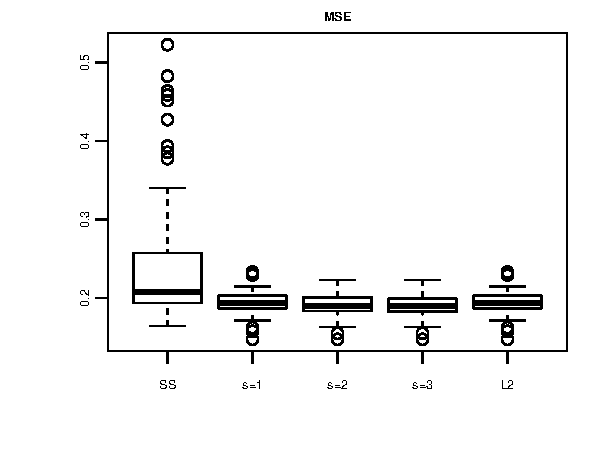
\includegraphics[height=0.3\textheight]{sim_results/sce=4_SNR=high_Kobs=30_MSE}
% 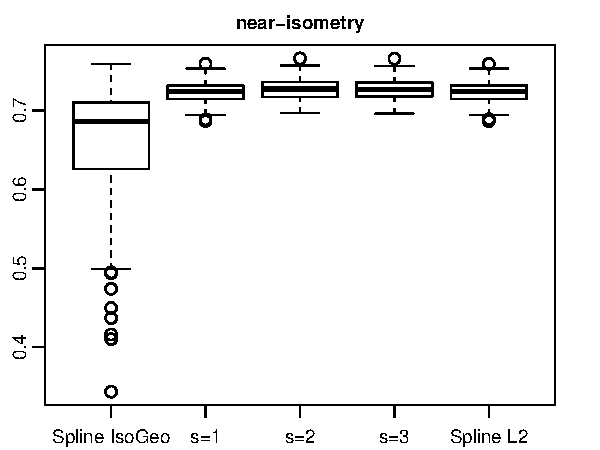
\includegraphics[height=0.3\textheight]{sim_results/sce=4_SNR=high_Kobs=30_isometry}
% 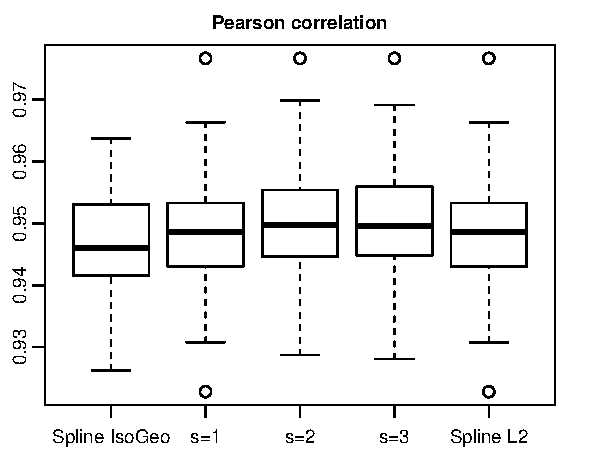
\includegraphics[height=0.3\textheight]{sim_results/sce=4_SNR=high_Kobs=30_Pearson}
% \caption{Manifold of square root Beta densities. Besides Spline IsoGeo, all methods perform comparably well.}
% \label{fig:betas}
% \end{figure}

\newpage

\bibliography{references}
\bibliographystyle{aaai}

\end{document}
